
    \Cref{chapter:theory} derived the underlying methodology for constraint
    programming on static single assignment compiler intermediate representation.
    Building on that framework, this chapter develops a domain specific
    constraint programming language and presents an implementation of this
    language within the production quality LLVM compiler infrastructure.

    The Compiler Analysis Description Language (CAnDL) automatically generates
    compiler analysis functionality that would otherwise have to be implemented
    manually.
    This fills an important niche in compiler development:
    Optimising compilers have to use elaborate program transformations to exploit
    increasingly complex hardware.
    Implementing the required analysis functionality for such optimizations to
    be safely applied is a time consuming and error prone activity.
    For example, tens of thousands of lines of code are required in the LLVM
    code base to detect the appropriate places to apply peephole optimizations,
    and bugs in this functionality can result in corrupted user programs.
    This is a barrier to the rapid prototyping and evaluation of new
    optimisations.

    CAnDL enables a workflow that is much more amenable to efficient compiler
    development.
    The compiler implementer only has to write CAnDL programs, which are then
    compiled by the CAnDL compiler fully automatically into C++ LLVM passes.
    These passes automatically spot code sections that adhere the specified
    structure, leaving only the transformation functionality to be implemented
    by hand.
    This provides a uniform manner in which to describe compiler analysis,
    significantly reducing code length and complexity.

    The approach scales to a wide range of compiler analysis tasks.
    Multiple case studies are presented that range from the detection of
    peephole optimisation opportunities, over domain specific graphics
    optimisations, to fully capturing static control flow regions for polyhedral
    code analysis.
    All these tasks can be  expressed more briefly than with competing
approaches.

\section{Introduction}

    Compilers are complex pieces of software responsible for the generation of
    efficient code.
    They transform input source code through several compilation stages,
    resulting in a binary program.
    In order to generate fast programs, modern compilers rely on a complex mid
    end.
    In this mid end, user code typically takes the form of a static single
    assignment intermediate representation and it is optimised by successively
    applying a wide range of optimisation passes.

    Most compiler optimisations require two steps:
    analysis and transformation.
    First, analysis routines find sections in user programs that enable the
    application of specific transformations.
    They further verify the necessary conditions to insure the transformation
    can be applied legally, without changing the program semantics.
    It is crucial that optimisations retain the semantics of the original
    program, as otherwise the resulting binary might be corrupted.
    Transformations are then applied to the analysis results in a second step.
    This often also involves heuristic cost models to gauge the effect on
    runtime, code size and other metrics.

    The complexity of the necessary analysis is an impediment to
    the implementation of new compiler passes, preventing the rapid
    prototyping of new ideas.
    For example, simple peephole optimisations in the LLVM {\tt instcombine}
    pass contain approximately 30000 lines of complex C++ code, despite the
    transformations being simple.
    Furthermore, this is an important source of bugs, and bugs in this stage of
    the compiler are particularly pernicious.
    They tamper with the user programs, but can remain unnoticed and often only
    trigger in corner cases.
    Ideally, there would be a simpler way of implementing such analysis that
    reduces boiler-plate code and opens the way for new compiler optimisation
    innovation.

    This chapter presents the Compiler Analysis Description Language (CAnDL), a
    domain specific language for compiler analysis.
    It is a constraint programming language, operating on the static single
    assignment intermediate representation of the LLVM compiler infrastructure
    (LLVM IR).
    Instead of writing compiler analysis code inside the main codebase of the
    compiler infrastructure, it enables compiler writers to specify optimization
    functionality external to the main C++ code base.
    The CAnDL compiler then generates C++ functions that are linked together
    with the clang compiler binary and that implement LLVM passes.
    The formulation of optimizing transformations in CAnDL is faster, simpler
    and less error prone than writing them in C++.
    It has a strong emphasis on modularity, which enables debugging and the
    formulation of highly readable code.

    CAnDL is based on the constraint programming methodology introduced in
    \Cref{chapter:theory}.
    It uses a solver that is integrated into the LLVM code base.
    CAnDL is developed as a complete programming language, with a full parser
    and code generator.
    The system is evaluated on a range of use cases from
    different domains, including: standard LLVM optimisation passes,
    custom optimisations for graphics shader programs and the detection static
    control flow regions for polyhedral program transformations.

\section{Motivating Example}

\begin{figure}[b]
\centering
\begin{minipage}[t]{0.67\textwidth}
\begin{lstlisting}[language=CAnDL]
Constraint SqrtOfSquare
( opcode{sqrt_call} = call
([$\tt \land$]) {sqrt_fn} = {sqrt_call}.args[0]
([$\tt \land$]) function_name{sqrt_fn} = sqrt
([$\tt \land$]) {square} = {sqrt_call}.args[1]
([$\tt \land$]) opcode{square} = fmul
([$\tt \land$]) {a} = {square}.args[0]
([$\tt \land$]) {a} = {square}.args[1])
End
\end{lstlisting}
\caption{The left side of \Cref{fig:root} as specified in CAnDL\parfillskip=0pt}
\label{fig:candlspec}
\end{minipage}
\end{figure}

    As an example of the CAnDL workflow, consider \Cref{fig:root}.
    This basic algebraic equation can be interpreted as a recipe for a compiler
    optimisation:
    Assuming an environment without the particularities of floating point
    arithmetic (i.e.\ assuming the \texttt{-ffast-math} flag is active), the
    compiler could use this equality to eliminate some square root invocations
    in user code.
    This is desirable, as the square root has to be approximated with relatively
    expensive numerical methods, whereas computing the absolute value is
    computationally cheap.
    \begin{align}
    \label{fig:root}
    \forall a\in \mathbb{R}\colon\ \sqrt{a*a}=|a|
    \end{align}

    The compiler should use the equation left to right:
    It should analyse the user code in order to find segments that correspond to
    the left side of the equation and then transform all those occurrences
    analogous to the right side of the equation.
    The compiler therefore must detect occurrences of $\sqrt{a*a}$ in the
    LLVM IR code and replace them with a call to the \texttt{abs} function.
    The generation of the new function call is trivial, but the detection of
    even this simple pattern requires some care when implementing it manually in
    a complex code base such as LLVM.

    The established approach in the clang compiler is to implement it in the
    \texttt{instcombine} pass, which applies a collection of such
    peephole optimisations and already extends to $\sim30000$ lines of
    C++ code.
    This code makes heavy use of raw pointers and dynamic type casts and has
    been identified as a frequent source of bugs, as documented by
    \citet{Yang:2011:FUB:1993316.1993532} and
    \citet{Menendez:2017:ADP:3062341.3062372}.
    This is impractical and an impediment to compiler development.

    Instead, CAnDL allows a declarative description of the analysis problem.
    It is easier to follow, has no interaction with other optimisations and
    is concise, as presented in \Cref{fig:candlspec}.
    The first line of the program assigns a name to the specification, which is
    then defined by the interaction of seven so-called {\em atomic constraint}s.
    These individual statements have to hold simultaneously on the values of
    \texttt{sqrt\_call}, \texttt{sqrt\_fn}, \texttt{square} and \texttt{a}.
    The lines 2--8 each stipulate one of these constraints, and they are joined
    together with logical conjunctions ``$\land$''.

    The CAnDL compiler translates the declarative program into a C++ function,
    which is then used for the analysis step in an LLVM optimisation pass.
    This is demonstrated in \Cref{fig:candlexample}, which shows the analysis
    function generated from the CAnDL specification in \Cref{fig:candlspec}
    applied to a user program as follows:
    The input program ({\bf a}) is a simple C function that calls the
    \texttt{sqrt} function twice with squares of floating point values.
    This is translated using the clang compiler into LLVM IR code ({\bf b}),
    applying standard optimisation passes during the process.
    The expression from the user program is here represented as a list of
    individual instructions and register assignments, with the two occurrences
    of \texttt{SqrtOfSquare} clearly visible:
    The two \texttt{fmul} instructions (lines 4 and 6) compute squares via a
    floating point multiplication, and these are then used as arguments to
    \texttt{sqrt} function invocations (lines 5 and 7).

    The optimised LLVM IR representation ({\bf b}) is used as the input to the
    generated analysis function, which detects two optimisation opportunities,
    identified as the first ({\bf c}) and second ({\bf d}) solutions of the
    constraint problem.
    Each of the two solutions assigns values from within the LLVM IR code to
    each of the variables in the CAnDL program in \Cref{fig:candlspec}, such
    that all the specified constraints are fulfilled.
    The validity of these solutions is demonstrated in the middle row of the
    figure ({\bf e}-{\bf f}).
    Substituting the variables in the CAnDL program with the concrete instances
    from the solutions, the individual atomic constraints can be verified
    individually:
    \begin{itemize}
    \item \texttt{\%4} and \texttt{\%6} are function calls and their first
          argument (the function to be called) is \texttt{@sqrt}.
    \item \texttt{@sqrt} is the square root function.
          Note that it is identified by name.
    \item The second arguments of the function call instructions (the first
          function arguments) are \texttt{\%3} and \texttt{\%5}
          respectively.
    \item \texttt{\%3} and \texttt{\%5} are square values, i.e.\ a floating
          point multiplication of a value with itself.
    \end{itemize}

    With the solutions identified by the CAnDL system, performing the
    transformation is now simple ({\bf g}).
    The solutions to the constraint problem are internally provided as C++
    dictionaries of the form \texttt{map<std::string,llvm::Value*>},
    containing all the information required to apply appropriate code
    transformations.
    A new function call to \texttt{abs} is generated, with \texttt{a} as the
    only argument (line 6).
    This instruction then replaces (line 4) the original call instruction that
    was captured in \texttt{sqrt\_call} (line 5).
    Conveniently, the LLVM infrastructure already provides all the necessary
    functions to create and replace instructions in the intermediate
    representation.
    After post processing with standard dead code elimination, this results in
    the optimised code shown at the bottom of the figure ({\bf h}).

    Although this is only a small example, it illustrates the main steps of the
    CAnDL scheme.
    In practice, the strength of the system is its ability to scale to very
    complex specifications, as demonstrated towards the end of the chapter.
    The next sections give a specification of the CAnDL language, and outline
    how it is implemented on top of the constraint programming methodology
    devised in \Cref{chapter:theory}.

\begin{figure*}[p]
    \centering
\begin{minipage}[t]{0.67\textwidth}
\centering
{\bf(a)} CAnDL program:
\begin{lstlisting}[language=CAnDL]
Constraint SqrtOfSquare
( opcode{sqrt_call} = call
([$\tt \land$]) {sqrt_call}.args[0] = {sqrt_fn}
([$\tt \land$]) function_name{sqrt_fn} = sqrt
([$\tt \land$]) {sqrt_call}.args[1]  = {square}
([$\tt \land$]) opcode{square} = fmul
([$\tt \land$]) {square}.args[0] = {a}
([$\tt \land$]) {square}.args[1] = {a})
End
\end{lstlisting}
\end{minipage}

\vspace{1em}
\begin{minipage}[t]{\textwidth}
\centering
\begin{minipage}[t]{\textwidth}
\centering
{\bf(b)} C program code:
\begin{lstlisting}[numbers=none,framexleftmargin=0pt,xleftmargin=0pt,language=C,basicstyle=\small\ttfamily]
 double example(double a, double b) {return sqrt(a*a) + sqrt(b*b); }
\end{lstlisting}
\end{minipage}
\begin{minipage}[t]{7.1cm}
\centering
{\bf(c)} Resulting LLVM IR:
\begin{lstlisting}[language={LLVM}]
define double @example(    
 double %0,                
 double %1) {              
 %3 = fmul double %0, %0   
 %4 = call double @sqrt(%3)
 %5 = fmul double %1, %1   
 %6 = call double @sqrt(%5)
 %7 = fadd double %4, %6   
 ret double %7 }
declare double @sqrt(double)      
\end{lstlisting}
\end{minipage}
\hfill
\begin{minipage}[t]{3.5cm}
\centering
{\bf(d)} First solution:
\begin{lstlisting}[numbers=none,framexleftmargin=0pt,xleftmargin=0pt,language=LLVM]

a = %0

square = %3
sqrt_call = %4 




sqrt_fn = @sqrt
\end{lstlisting}
\end{minipage}
\hfill
\begin{minipage}[t]{3.5cm}
\centering
{\bf(e)} Second solution:
\begin{lstlisting}[numbers=none,framexleftmargin=0pt,xleftmargin=0pt,language=LLVM]


a = %1


square = %5
sqrt_call = %6


sqrt_fn = @sqrt
\end{lstlisting}
\end{minipage}
\end{minipage}


\vspace{1em}
\begin{minipage}[t]{\textwidth}
\centering
{\bf(f)} C++ transformation code:
\begin{lstlisting}
void transform(map<string,Value*> solution, Function* abs) {
    ReplaceInstWithInst(
       dyn_cast<Instruction>(solution["sqrt_call"]),
       CallInst::Create(abs, {solution["a"]}));
}
\end{lstlisting}
\end{minipage}

\vspace{1em}
\begin{minipage}[t]{\textwidth}
\centering
{\bf(g)} Transformed LLVM IR after DCE:
\begin{lstlisting}[escapeinside={(*}{*)},language={LLVM}]
define double @example(double %0, double %1) {              
 %3 = call double @abs(double %0) 
 %4 = call double @abs(double %1)
 %5 = fadd double %3, %4   
 ret double %5 }
\end{lstlisting}
\end{minipage}

\caption{Demonstration of a simple CAnDL specification ({\bf a}) on an example C
         program ({\bf b}):
         In the generated LLVM intermediate code ({\bf c}), two instances
         ({\bf d},{\bf e}) of {\tt SqrtOfSquare} are detected.
         Applying an optimization using these results is trivial ({\bf g}) and
         results in efficient code ({\bf e}).}
    \label{fig:candlexample}
\end{figure*}

\section{Language Specification}

    The Compiler Analysis Description Language is a domain specific
    programming language for the specification of compiler analysis problems. 
    Individual CAnDL programs define specific computational structures that
    exist in user programs and that can be exploited by applying code
    transformations.
    These structures are specified as constraint programs on the LLVM IR
    representations of user code.
    CAnDL builds on generic concepts from \Cref{chapter:theory}.
    These are independent of LLVM, so the methodology translates to other SSA
    representations.

    The expressed structures can scale from simple instruction patterns that are
    suited for peephole optimizations, over control flow structures such
    as loops, to complex algorithmic concepts such as code regions that are
    suitable for polyhedral code transformations.

    Like traditional constraint programs, CAnDL programs have two
    fundamental features: \textbf{variables} and \textbf{constraints}.
    The basic constraint building blocks are well established compiler analysis
    tools, such as constraints on data and control flow, data types and
    instruction opcodes.
    These are composed with logical connectors and several higher level language
    features, such as range expressions, with finally a system of modularity and
    extensibility on top.
    This section introduces the language features, starting from the overall
    program structure.

\subsection{High-Level Structure of CAnDL Programs}

    The following notational conventions are used for the description of CAnDL
    syntax in this section:
    terminal symbols are {\bf bold}, non-terminals are {\it italic},
    $\left<\text{\bf s}\right>$ is an identifier (alphanumeric string) and
    $\left<\text{\bf n}\right>$ is an integer literal.
    CAnDL uses Unicode characters such as ``$\land$'', ``$\in$'', ``$\Phi$'' and
    is encoded as UTF-8.
    An individual CAnDL program contains constraint formulas that are
    bound to identifiers.
    As previously shown in \Cref{fig:candlspec}, the syntax for this is as
    follows:
\begin{figure}[H]
\centering
\begin{tabular}{|c|}
    \hline
    $specification ::= \text{\bf Constraint}\ \left<\text{\bf s}\right>\ \text{\it formula}\ \text{\bf End}$\\
    \hline
\end{tabular}
\end{figure}

    \noindent
    Furthermore, \Cref{fig:candlspec} already demonstrated how logical
    conjunctions are used to combine simpler {\it formula}s.
    More generally, a {\it formula} can be any of the following:
\begin{figure}[H]
\centering
\begin{tabular}{|c|}
    \hline
    $formula ::= \text{\it atomic}\mid\text{\it conjunction}\mid\text{\it disjunction}\mid\text{\it foreach}\mid \text{\it forany}\mid\text{\it include}\mid\text{\it collect}$\\
    \hline
\end{tabular}
\end{figure}

    \noindent
    The basis of every CAnDL program are {\it atomic} constraints, which are
    bound together by logical connectives ``$\land$'' and ``$\lor$''
    ({\it conjunction} and {\it disjunction}), as well as other higher level
    constructs.
    These include two kinds of range structures ({\it foreach}, {\it forany}),
    and a system for modularity ({\it include}).
    Lastly, the {\it collect} construct allows for the formulation of more
    complex constraints that require the $\forall$ quantifier.
    The individual classes of atomic constraints are introduced next,
    followed by the higher level constructs.

\subsection{Atomic Constraints}

\begin{figure}[t]
  \centering
  \begin{tabular}{|c|c|}
    \hline
    syntax & SSA model formulation \\
    \hline
    \hline
    $\text{\bf data\_type}\ \text{\it variable}\ \text{\bf =}\ \left<\text{\bf s}\right>$ &  $(s,x)\in T_\mathcal F$\\
    \hline
    $\text{\bf ir\_type}\ \text{\it variable}\ \text{\bf =}\ \text{\bf literal}$ &  $x\in C_\mathcal F^*$\\
    $\text{\bf ir\_type}\ \text{\it variable}\ \text{\bf =}\ \text{\bf argument}$ & $x\in P_\mathcal F^*$\\
    $\text{\bf ir\_type}\ \text{\it variable}\ \text{\bf =}\ \text{\bf instruction}$ & $x\in I_\mathcal F^*$\\
    \hline
    $\text{\bf opcode}\ \text{\it variable}\ \text{\bf =}\ \left<\text{\bf s}\right>$ & $(s,x)\in I_\mathcal F$\\
    \hline
    $\text{\bf function\_name}\ \text{\it variable}\ \text{\bf =}\ \left<\text{\bf s}\right>$ & $(\text{!name=}s,x)\in T_\mathcal F$\\
    \hline
  \end{tabular}
  \caption{The simplest atomic constraints operate on a single variable and
           check element-of properties for the different sets in the SSA model.
           Function names are accommodated in $T_\mathcal F$.\parfillskip=0pt}
  \label{onevaratomics}
\end{figure}

\begin{figure}[t]
  \centering
  \begin{tabular}{|c|c|}
    \hline
    syntax & SSA model formulation \\
    \hline
    \hline
    $\text{\it variable}\ \text{\bf =}\ \text{\it variable}\text{\bf.args[}\left<\text{\bf n}\right>\text{\bf]}$ & $(n,x,y)\in DFG_\mathcal F$\\
    $\text{\it variable}\ \text{\bf $\in$}\ \text{\it variable}\text{\bf .args}$ & $(x,y)\in DFG_\mathcal F^*$\\
    \hline
    $\text{\it variable}\ \text{\bf =}\ \text{\it variable}\text{\bf.successors[}\left<\text{\bf n}\right>\text{\bf]}$ & $(n,y,x)\in CFG_\mathcal F$\\
    $\text{\it variable}\ \text{\bf $\in$}\ \text{\it variable}\text{\bf .successors}$ & $(y,x)\in CFG_\mathcal F^*$\\
    \hline
    $\text{\it variable}\ \text{\bf =}\ \text{\it variable}$ & $x=y$\\
    $\text{\it variable}\ \text{\bf !=}\ \text{\it variable}$ & $x\neq y$\\
    \hline
  \end{tabular}
  \caption{The second class of atomic constraints operate on pairs of variables.
           The constraints check for graph edges in the
           data flow and control low graphs, or simply for shallow equivalence.
           \parfillskip=0pt}
  \label{twovaratomics}
\end{figure}

    Based on the SSA model from \Cref{chapter:theory}, CAnDL provides a wide
    range of atomic constraints.
    The simplest group are those that operate on only a single variable,
    listed in \Cref{onevaratomics}.
    They operate immediately on the underlying mathematical structures, testing
    element-of properties of the sets in order to constrain data types,
    instruction opcodes etc.
    At the bottom of the list is the {\bf function\_name} constraint,
    which is particular.
    Function names are not a fundamental component of the SSA model from
    \Cref{chapter:theory}.
    However, they are easily accommodated within the type information
    $T_\mathcal F$.
    The same data structure can also be used to capture all kinds of LLVM
    specific metadata.

    There are additional atomic constraint that operate on pairs of variables.
    These are listed in \Cref{twovaratomics}.
    These most importantly check for edges in the control flow and data flow
    graphs.
    Furthermore, two constraints are available for shallow comparisons of
    variables.


%\begin{figure}[h]
%  \centering
%  \begin{tabular}{|c|c|}
%    \hline
%    syntax & SSA model formulation \\
%    \hline
%    \hline
%    \multirow{2}{*}{$\text{\it variable}\ \text{\bf ->}\ \text{\it variable}\ \Phi\ \text{\it variable}$}
%        & $(z,phi)\in I_\mathcal F\mathrel\land (y,z)\in m(CFG_\mathcal F^*)\mathrel\land$ \exists n: \\
%        & $(x,z,n)\in DFG_\mathcal F\mathrel\land n=|\{y'\leq y\mid (y',z)\in m(CFG_\mathcal F^*)\}|$\\
%    \hline
%  \end{tabular}
%  \caption{CAnDL exposes Phi nodes with a dedicated atomic constraint.
%           The modified control flow graph $m(CFG_\mathcal F^*)$ duplicates
%           control flow edges into basic blocks with multiple Phi nodes.}
%  \label{phiatomic}
%\end{figure}

    Besides those constraints that operate immediately on the sets of the
    SSA model, there are several atomic constraints that enforce graph
    properties.
    This includes dominance relationships and the interaction of data flow and
    control flow for $\Phi$-instructions.

%    \begin{align*}
%        \text{\bf control\_origin}&\ \text{\it variable}\\
%        \text{\bf data\_origin}&\ \text{\it variable}
%    \end{align*}
%    The value is an origin of control (function entry) or data (function argument, {\tt load} instruction, inpure function call).

\subsubsection{Phi Nodes}

    The following syntax is used to express the condition that a value has to
    reach a $\Phi$-instruction via a specific jump instruction:
\begin{figure}[h]
    \centering
    \begin{tabular}{|c|}
        \hline
        $\text{\it variable}\ \text{\bf ->}\ \text{\it variable}\ \Phi\ \text{\it variable}$\\
        \hline
    \end{tabular}
\end{figure}

    \noindent
    More precisely, the expression $\{A\}\text{\bf ->}\{B\}\Phi\{C\}$ means that
    the value of $C$ is $A$ if $B$ was the last branch taken before $C$ was
    reached.
    Using the SSA model, this is equivalent to the following:
    \begin{align*}
        (C,phi)\in I_\mathcal F\mathrel\land{}&(B,h(C))\in CFG_\mathcal F^*\mathrel\land(A,C,n)\in DFG_\mathcal F,\\
            \text{where }h(C):={}&min\{c\mid (phi,x)\in I_\mathcal F\text{ for all }c\leq x\leq C\}\\
            \text{and }n:={}&\{b\leq B\mid (b,h(C))\in CFG_\mathcal F^*\}.
    \end{align*}
    Firstly, $C$ is a $\Phi$-instruction.
    Secondly, $B$ has a control flow edge to the basic block containing $C$.
    The first instruction of this basic block is identified as $h(C)$, to
    account for the possibility of more than one $\Phi$-instruction in the
    basic block.
    Thirdly, $A$ is the $n$th argument of $C$, where $n$ is the index of $B$ in
    the list of jump instructions that target $h(C)$.

\subsubsection{Graph Domination}

    In order to express domination in the control flow graph, the following
    syntax is used:
\begin{figure}[h]
    \centering
    \begin{tabular}{|c|}
        \hline
        $\text{\bf domination(}\text{\it variable}\text{\bf,} \text{\it variable}\text{\bf)}$\\
        $\text{\bf strict\_domination(}\text{\it variable}\text{\bf,} \text{\it variable}\text{\bf)}$\\
        \hline
    \end{tabular}
\end{figure}

    \noindent
    For both these constraints, the values are implicitly limited to
    instructions.
    The expression ``{\bf domination}(\{A\},\{B\})'' means that $A$ is a
    dominator of $B$, i.e.\ any path through the control flow graph from the
    entry node to $B$ must go through $A$.
    Strict domination additionally requires that $A$ and $B$ are distinct.

    Completing the domination constraints, there are corresponding
    post-dominator versions {\bf post\_domination} and
    {\bf strict\_post\_domination}, as well as the following generalisation:
\begin{figure}[h]
    \centering
    \begin{tabular}{|c|}
        \hline
        ${\bf all}\ {\bf control}\ {\bf flow}\ {\bf from}\ variable\ {\bf to}\ variable\ {\bf passes}\ {\bf through}\ variable$\\
        \hline
    \end{tabular}
\end{figure}

    \noindent
    This constraint is similar to a standard control flow domination, but
    instead of taking paths from the control flow origin, a third variable is
    used for parametrisation. 
%    \begin{align*}
%        \text{\bf calculated\_from(}\text{\it varlist}\text{\bf,}\text{\it varlist}\text{\bf,}\text{\it variable}\text{\bf)}
%    \end{align*}
%    {\it Varlist} is a set of one or multiple {\it variables}.
%    Any path from one of the entries in the first {\it varlist} to the single
%    {\it variable} argument has to pass through at least one of the entries in
%    the second {\it varlist}.
%    All paths in the union of the data flow and control dependence graph are
%    considered.
%    We will see later how this is useful to specify kernel functions for
%    e.g.\ stencil calculations.

\subsubsection{Additional Atomic Constraints}

    The set of atomic constraints that are supported by CAnDL can easily be
    extended.
    Possible additions include constraints on function attributes and value
    constraints on literals.
    This will be further explored in the later
    \Cref{chapter:reductions,chapter:idioms}.

\subsection{Range Constraints}

\begin{figure}[t]
\begin{lstlisting}[language=CAnDL]
Constraint ValueChain
 {element[i] ([$\tt \in$]) {element[i+1]}.args foreach i=0..4
End
\end{lstlisting}
\begin{lstlisting}[language=CAnDL]
Constraint ValueChain
( {element[0]} ([$\tt \in$]) {element[1]}.args
([$\tt \land$]) {element[1]} ([$\tt \in$]) {element[2]}.args
([$\tt \land$]) {element[2]} ([$\tt \in$]) {element[3]}.args
([$\tt \land$]) {element[3]} ([$\tt \in$]) {element[4]}.args)
End
\end{lstlisting}
\caption{Example for the expansion of range constraints in CAnDL:
         The specification at the top can be ``unrolled'' manually,
         resulting in the equivalent, but more verbose, specification below.
         \parfillskip=0pt}
\label{fig:forall}
\end{figure}

    Building on top of the atomic constraints and the fundamental conjunction
    and disjunction constructs, there are range based constraints that operate
    on arrays of variables:
\begin{figure}[h]
  \centering
  \begin{tabular}{|c|}
    \hline
    $foreach ::= \text{\it formula}\ \text{\bf foreach}\ \left<\text{\bf s}\right>\ \text{\bf =}\ \text{\it index}\ \text{\bf ..}\ \text{\it index}$\\
    $forany ::= \text{\it formula}\ \text{\bf forany}\ \left<\text{\bf s}\right>\ \text{\bf =}\ \text{\it index}\ \text{\bf ..}\ \text{\it index}$\\
    \hline
  \end{tabular}
\end{figure}

    \noindent
    These constructs allow the replication of a constraint formula over a range
    of indices.
    This is demonstrated in \Cref{fig:forall}, which shows two equivalent
    CAnDL programs, the first one formulated with {\it foreach} and the
    second one without.
    In both cases, the program specifies an array of five variables with data
    flow from each element to the next.
    This shows how {\it foreach} can be expanded by duplicating the contained
    formula, with logical conjunctions binding the replicas of the
    formula together.
    Otherwise identical, the {\it forany} construct is based on logical
    disjunctions instead.

    The syntactic structure of variable identifiers carries no semantic
    information for atomic constraints.
    This is clearly not true for range expressions, which rely on index
    calculations in order to evaluate the underlying variables.
    Therefore, it is important to now introduce the precise syntax for variable
    names, which are constructed as follows:

\begin{figure}[h]
  \centering
  \begin{tabular}{|c|}
    \hline
    $variable ::= \left<\text{\bf s}\right>\mid\text{\it variable}\ \text{\bf [}\ \text{\it calculation}\ \text{\bf ]}\mid\text{\it variable}\ \text{\bf.}\ \left<\text{\bf s}\right>$\\
    $calculation ::= \left<\text{\bf s}\right>\mid\left<\text{\bf n}\right>\mid\text{\it calculation}\ \text{\bf+}\ \text{\it calculation}\mid\text{\it calculation}\ \text{\bf-}\ \text{\it calculation}$\\
    \hline
  \end{tabular}
\end{figure}

    \noindent
    The syntax of variable identifiers in CAnDL aligns closely to C/C++
    conventions.
    They can contain simple index calculations to support the range constructs,
    as well as a hierarchical structure.
    This hierarchical structure corresponds to the modularity capabilities of
    CAnDL that are introduced in the next section.

\subsection{Modularity}

    Modularity is central to CAnDL, and it is achieved using the {\it include}
    construct.
    \begin{figure}[h]
        \centering
        \begin{tabular}{|c|}
            \hline
            $\text{\bf include}\ \left<\text{\bf s}\right>
                                [\ \text{\bf (}\text{\it variable}\ \text{\bf ->}\ \text{\it variable}\ \{\ \text{\bf ,}\ \text{\it variable}\ \text{\bf ->}\ \text{\it variable}\ \}\ \text{\bf )}\ ]\ 
                                [\ \text{\bf @}\ \text{\it variable}\ ]$\\
            \hline
        \end{tabular}
    \end{figure}

    \noindent
    Note that the syntax in square brackets ``[]'' is optional and the syntax in
    curly brackets ``\{\}'' may be repeated.
    The basic version of \texttt{\it include}, using none of the optional
    structures, is simple.
    It copies the formula that corresponds to the identifier verbatim into
    the current specification.
    If ``$[\text{\bf @}\ \text{\it variable}]$'' is specified, then all the
    variable names of the inserted constraint formula are prefixed with the
    given variable name, separated with a dot.
    The other optional syntax is used to rename individual variables in
    the included formula.
    If both optional constructs are used together, then the prefix is only
    applied to variables that are not renamed.

    \Cref{fig:inheritsandrenameandrebase} illustrates this with two
    equivalent constraint programs.
    Both programs specify an addition of four values, first adding pairwise and
    then adding the intermediate results.
    In the first listing, a formula for the addition of two values is
    bound to the name {\tt Sum}.
    This is then included three times in another formula named {\tt SumOfSums}.
    Using the optional grammatical constructs, the formula operates on a
    different set of variables each time, such that the third addition
    takes the results of the previous two as input.

\begin{figure}[h]
\lstset{
 basicstyle = \linespread{0.88}\ttfamily
}
\begin{lstlisting}[language=CAnDL]
Constraint Sum
( opcode{out} = add
∧ {in1} = {out}.args[0]
∧ {in2} = {out}.args[1])
End
Constraint SumOfSums
( include Sum@{sum1}
∧ include Sum@{sum2}
∧ include Sum({sum1.out}->{in1},{sum2.out}->{in2}))
End
\end{lstlisting}
\begin{lstlisting}[language=CAnDL,
                   label={fig:inheritsandrenameandrebase},caption=
   {Example for the expansion of {\it include} structure:
    Both specifications are equivalent.
    \leftskip=0pt\rightskip=0pt}]
Constraint SumOfSums
( opcode{sum1.out} = add
∧ {sum1.in1} = {sum1.out}.args[0]
∧ {sum1.in2} = {sum1.out}.args[1]
∧ opcode{sum2.out} = add
∧ {sum2.in1} = {sum2.out}.args[0]
∧ {sum2.in2} = {sum2.out}.args[1]
∧ opcode{out} = add
∧ {sum1.out} = {out}.args[0]
∧ {sum2.out} = {out}.args[1])
End
\end{lstlisting}
\caption{Example for the expansion of {\it include} constraints:
         Both specifications are equivalent.\parfillskip=0pt}
\label{fig:inheritsandrenameandrebase}
\end{figure}

\subsubsection{Collect}

    The \text{\it collect} construct captures all possible solutions of a given
    formula.
    It is used to implement constraints that require logical quantifiers
    $\forall$ (``for all'') and $\exists$ (``there exists some'').
%    For example, it can guarantee that all memory accesses in a loop use affine
%    index computations.
%    The grammar is simple but the semantics require some elaboration.
\begin{figure}[H]
    \centering
    \begin{tabular}{|c|}
        \hline
        $\text{\bf collect}\ \left<\text{\bf s}\right>\ \text{\it index}\ \text{\it formula}$\\
        \hline
    \end{tabular}
\end{figure}

    \noindent
    In \Cref{fig:simplecollect}, the variables \texttt{arg[0],\dots,arg[N-1]}
    are constrained to contain all of the direct data dependences of
    \texttt{ins}.
    The first argument of \text{\it collect} specifies the name of an index
    variable that is used to detect which variables belong to the collected set.
    In this example, solutions of \texttt{arg[i]} for a given value
    of \texttt{ins} are identified.
    The second argument gives an upper bound to the amount of collected
    variables.
    It is left unspecified in this case by using the symbol \texttt{N}.

\begin{figure}[t]
\begin{lstlisting}[language=CAnDL]
Constraint CollectArguments
( ir_type{ins} = instruction
([$\tt \land$]) collect i N ({arg[i]} ([$\tt \in$]) {ins}.args))
End
\end{lstlisting}
\caption{Simple {\it collect} example in CAnDL: All direct data dependences of
         {\tt ins} are collected.}
\label{fig:simplecollect}
\end{figure}

    This example is now extended to show how {\it collect} can be used to
    implement quantifiers.
    Consider that the aim is to detect instructions with only floating point
    direct data dependences.
    This involves the $\forall$ quantifier, as it is equivalent to
    the following equation:
    \begin{align}
        \forall x\colon\ (x,ins)\in DFG_\mathcal F^*\implies(float,x)\in I_\mathcal F
        \label{fig:implication}
    \end{align}
    This can be rewritten to an equivalent formulation on sets:
    \begin{align*}
        S_1:= select(ins,rev(DFG_\mathcal F^*))\subset S_2:=select(float,I_\mathcal F).
    \end{align*}

    Using the equivalence
    $S_1\subset S_2\iff S_1 = S_1\cap S_2$, this means that
    if a set $S$ is constrained to be equal to both $S_1$ and $S_1\cap S_2$,
    these constraints are satisfiable if and only if the implication in
    \Cref{fig:implication} holds.
    This condition can be expressed in CAnDL, as is shown in
    \Cref{fig:collectexample}.
    With the first {\it collect} statement in line 3, the set \texttt{arg} is
    constrained to be equal to $S_1$ and with the second one in lines 4-5, it
    is constrained to be $S_1\cap S_2$ as well.

\begin{figure}[H]
\begin{lstlisting}[language=CAnDL]
Constraint FloatingPointInstruction
( ir_type{ins} = instruction
([$\tt \land$]) collect i N ( {ins} ([$\tt \in$]) {arg[i]}.args)
([$\tt \land$]) collect i N ( {ins} ([$\tt \in$]) {arg[i]}.args
              ([$\tt \land$]) data_type{arg[i]} = float))
End
\end{lstlisting}
\caption{{\it Collect} is used to constrain {\tt ins} to be calculated from only
         floating point values.}
\label{fig:collectexample}
\end{figure}

    The exact same approach can be used for much more complex analysis tasks.
    For example, the final case study at the end of this chapter uses
    {\it collect} statements to restrict all array accesses within a
    loop to be affine in the loop iterators:
    First {\it collect} all memory accesses in the loop
    (i.e.\ all \texttt{load} and \texttt{store} instructions), and then use a
    second {\it collect} statement to enforce affine calculations of the access
    indices that are used by the address calculations for these instructions.

\subsection{Expressing Larger Structures}

\begin{figure}[p]
\begin{lstlisting}[language=CAnDL,basicstyle=\linespread{0.78}\ttfamily]
Constraint SESE
( opcode{precursor} = branch
([$\tt\land$]) {begin} ([$\tt\in$]) {precursor}.successors
([$\tt\land$]) opcode{end} = branch
([$\tt\land$]) {successor} ([$\tt\in$]) {end}.successors
([$\tt\land$]) domination({begin}, {end})
([$\tt\land$]) post_domination({end}, {begin})
([$\tt\land$]) strict_domination({precursor}, {begin})
([$\tt\land$]) strict_post_domination({successor}, {end})
([$\tt\land$]) all control flow from {begin} to {precursor}
         passes through {end}
([$\tt\land$]) all control flow from {successor} to {end}
         passes through {begin}) End
\end{lstlisting}
\caption{Single entry single exit region in CAnDL:
         The region spans from {\tt begin} to {\tt end}, with the entry as
         control flow {\tt precursor} to {\tt begin}, and the exit as control
         flow {\tt end} to {\tt successor}.
         \parfillskip=0pt}
\label{fig:CAnDLSESE}
\end{figure}

\begin{figure}[p]
\begin{lstlisting}[language=CAnDL,basicstyle=\linespread{0.78}\ttfamily]
Constraint Loop
( include SESE
([$\tt\land$])  {begin} ([$\tt\in$]) {end}.successors) End
\end{lstlisting}
\caption{Loops are defined in CAnDL as single entry single exit regions with a
         back edge.
         The back edge does not break the ``single exit'' condition, because it
         does not exit the region.
         \parfillskip=0pt}
\label{fig:CAnDLLoop}
\end{figure}

\begin{figure}[p]
\begin{lstlisting}[language=CAnDL,basicstyle=\linespread{0.78}\ttfamily]
Constraint LocalConst
( ir_type{value} = literal
([$\tt\lor$]) ir_type{value} = argument
([$\tt\lor$]) strict_domination({value}, {loop.begin})) End
\end{lstlisting}
\caption{This specification restricts {\tt value} to remain constant during
         the execution of a loop.
         It is underspecified on its own, and should be included in
         larger CAnDL programs that also include {\tt Loop},
         renaming {\tt value} to the specific variable that needs to be constrained in this way.
         \parfillskip=0pt}
\label{fig:localconstant}
\end{figure}

\begin{figure}[p]
\begin{lstlisting}[language=CAnDL,basicstyle=\linespread{0.78}\ttfamily]
Constraint PointerAccess
( ( (opcode{access} = store ([$\tt \land$]) {pointer} = {access}.args[1])
  ([$\tt \lor$]) (opcode{access} = load  ([$\tt \land$]) {pointer} = {access}.args[0]))
([$\tt \land$]) domination({loop.begin}, {access})
([$\tt \land$]) post_domination({loop.end}, {access})) End

Constraint ArrayAccess
( include PointerAccess
([$\tt \land$]) opcode{pointer} = getelementptr
([$\tt \land$]) {base_pointer} = {pointer}.args[0]
([$\tt \land$]) include LocalConst({base_pointer}->{value})) End

Constraint LoopWithOnlyArrayAccesses
( include Loop
([$\tt \land$]) collect i N (include PointerAccess({}->{loop})@acc[i])
([$\tt \land$]) collect i N (include ArrayAccess({}->{loop})@acc[i])) End
\end{lstlisting}
\caption{Building blocks are combined to restrict the allowed memory accesses
         of a loop.
         \leftskip=0pt\rightskip=0pt}
\label{fig:arrayloop}
\end{figure}

    The modularity of CAnDL allows for the creation of building blocks that are
    used by multiple CAnDL specifications.
    This includes classic control flow structures, such as single entry single
    exit (SESE) regions and different classes of loops, as well as memory access
    patterns.
    They form a standard library that enables higher-level programming
    within CAnDL.
    This section gives an overview of how some of these standard building
    blocks are defined.

    \Cref{fig:CAnDLSESE} gives the specification of SESE regions in CAnDL.
    Such regions are spanned by the variables {\tt begin} and {\tt end}, with an
    incoming control flow edge from {\tt precursor} to {\tt begin} (line 3) and
    an outgoing control flow edge from {\tt end} to {\tt successor} (line 5).
    Graph domination constraints in lines 8 and 7 guarantee that these are the
    only entry and exit of the region.
    Additional domination constraints in lines 6--7 and lines 10--13 make sure
    that there are no jumps from outside the region into an instruction of the
    region that is not {\tt begin}, and similarly that there are no early exits
    of the region.
    Finally, regions are restricted to align with basic block boundaries in
    lines 2 and 4.

    Natural loops are easily defined in CAnDL, as is visible in
    \Cref{fig:CAnDLLoop}.
    The specification includes {\tt SESE}, and adds only a single additional
    constraint for the back edge of the loop in line~3.
    Additional extensions to this specification are added to define more
    restricted loop structures, such for loops.
    This involves the identification of the loop iterator, the breaking
    condition, and the corresponding iteration space boundaries.
    In order to be a valid for loop, the end of the iteration space has to be
    determined before the loop is entered.
    This is expressed in \Cref{fig:localconstant}, restricting {\tt value}
    to be either a function argument, a constant or an instruction that strictly
    dominates the loop entry.
    Note that this formula is underspecified on its own.
    It is to be included into larger CAnDL programs that also include
    {\tt Loop}.

    Another class of important building blocks are different categories of
    memory access.
    These form a hierarchy of restrictiveness and include multidimensional array
    access and array access that is affine in some loop iterators.
    \Cref{fig:arrayloop} combines several of the introduced building blocks to
    specify a loop in which all memory access locations are calculated as
    offsets from base pointers that are constant within the loop.
    This for example excludes loops with pointer chasing.
    The {\tt ArrayAccess} specification can be extended with more restrictive
    memory access patterns as previously mentioned.
    This is crucial to define advanced compiler analysis passes, such as the
    detection of regions suitable for polyhedral code analysis.

\begin{figure}[t]
\centering
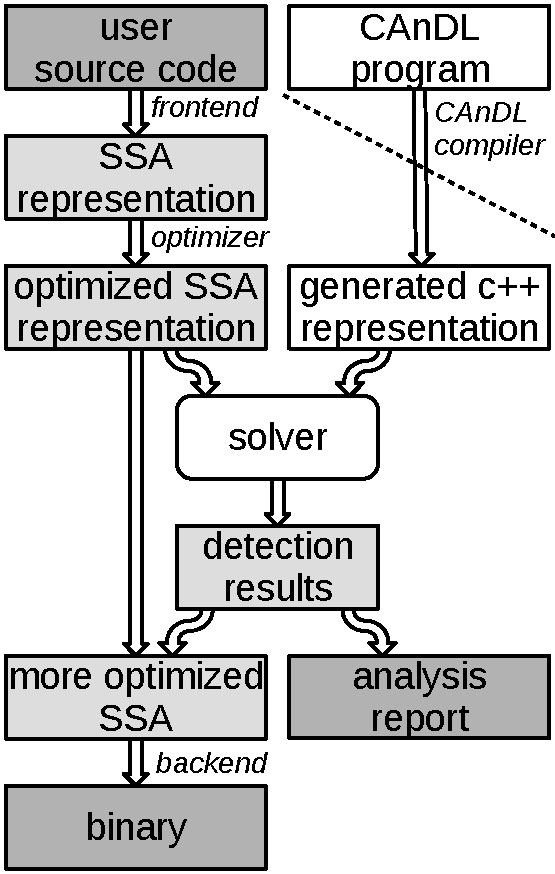
\includegraphics[width=0.59\textwidth]{figures/compilerFlow2.pdf}
\caption{CAnDL in the LLVM/clang system: The CAnDL code gets parsed by the
         CAnDL compiler and turned into C++, which is compiled directly
         into LLVM and then used by clang.
         \parfillskip=0pt}
\label{fig:build2}
\end{figure}

\section{Implementation}

    CAnDL is embedded in the LLVM framework, as shown in \Cref{fig:build2}.
    CAnDL programs are read by the CAnDL compiler during LLVM build time, which
    then generates C++ source code to implement the specified LLVM analysis
    functionality.
    This code depends on the generic backtracking solver derived in
    \Cref{chapter:theory}, which is incorporated directly into the LLVM code
    base.
    The generated code is compiled and linked together with the existing LLVM
    libraries.
    The clang compiler, which is built on LLVM, then automatically invokes this
    solver during the compilation of user programs, after the standard
    optimisation passes.
    The evaluation at the end of the chapter will show that this solver adds
    little compile-time overhead in practice.

    The resulting modified version of the clang compiler uses the solver to
    search for the specified computational structures and outputs the found
    instances into report files.
    It also makes the results available to ensuing transformation passes in the
    form of C++ structures.

\subsection{The CAnDL Compiler}

\begin{figure}[t]
\centering
\begin{minipage}{0.7\textwidth}
\centering
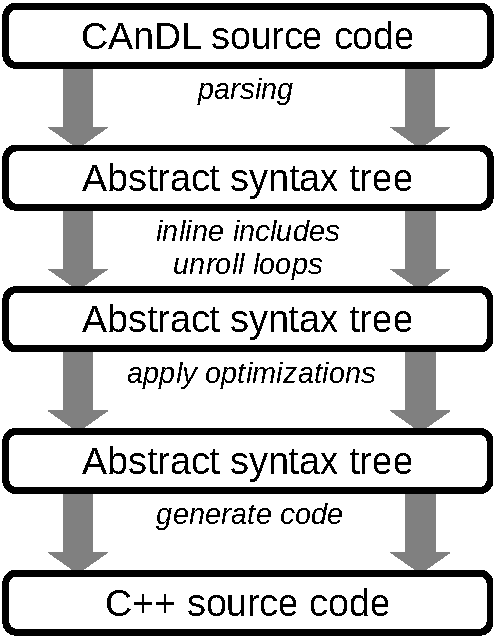
\includegraphics[width=0.85\textwidth]{figures/candlstages.pdf}
\caption{Flow within the CAnDL compiler:
         The CAnDL source code gets lowered in several steps to generated C++
         source code.\parfillskip=0pt}
\label{fig:compilerflow}
\end{minipage}
\end{figure}

    The CAnDL compiler is responsible for parsing CAnDL programs and
    generating C++ code from them.
    An overview of its  flow is shown in \Cref{fig:compilerflow}.
    The frontend reads in  CAnDL source code and builds an abstract syntax tree.
    This syntax tree is simplified in two steps to eliminate some of the higher
    order constructs of CAnDL.
    The {\it inheritance} clauses are inlined after the contained variables
    have been transformed accordingly.
    Also, {\it foreach} and {\it forany} statements are lowered to
    conjunction and disjunction constructs by duplicating the contained
    constraint code and then renaming its variables appropriately
    for each iteration.
    The remaining core language now consists only of atomics, conjunctions,
    disjunctions and collections.

    The CAnDL compiler then applies a set of optimisations to speed up the
    solving process using the later generated C++ code.
    For example, nested conjunctions and disjunctions are flattened wherever
    possible.
    Furthermore, if shallow equivalence of two variables is enforced in a
    conjunction, one of the two variables is chosen as having higher priority.
    all occurrences of the other variable are then replaced with that one.

    Finally, the compiler generates C++.
    This essentially means generating a function which at runtime constructs
    the constraint problem as a graph structure that is accessible to the
    solver.

\subsubsection{C++ Code Generation}

\begin{figure}[t]
\centering
\begin{lstlisting}[language=CAnDL]
Constraint SimpleAddition
( opcode{addition} = add
([$\tt \land$]) {addition}.args[0] = {left}
([$\tt \land$]) {addition}.args[1] = {right})
End
\end{lstlisting}
\begin{lstlisting}[language=C++]
auto constr0 = make_shared<AddInstruction>(model);
auto constr1 = make_shared<FirstArgument> (model);
auto constr2 = make_shared<SecondArgument>(model);
auto constr3 = make_shared<Conjunction>(
                   constr0,
                   select<0>(constr1),
                   select<0>(constr2));

vector<pair<string,shared_ptr<BacktrackingPart>>> result(3);
result[0] = make_pair("addition", constr3);
result[1] = make_pair("left",     select<1>(constr1));
result[2] = make_pair("right",    select<1>(constr2));
\end{lstlisting}
\caption{C++ source code generation}
\label{fig:codegen}
\end{figure}

    The code generation process is demonstrated in \Cref{fig:codegen} with an
    example.
    Each of the atomic constraints results in a line of C++ code that constructs
    an object of a corresponding class:
    In this case, the three involved atomic constraints are implemented by
    \texttt{AddInstruction}, \texttt{FirstArgument} and \texttt{SecondArgument}.
    For constraints that 
    These objects are instantiated as shared pointers.

    The compiler then generates similar objects for the
    \texttt{conjunction}, \texttt{disjunction} and the \texttt{collect} structures.
    In our example, this only affects the variable \texttt{addition}, which is
    part of a \texttt{conjunction} clause.
    This results in an additional object construction that instantiates the
    \texttt{Conjunction} class corresponding to the ``$\land$'' operator
    in CAnDL.

    Those constraint classes that implement constraints on a single variable
    directly implement the \texttt{BacktrackingPart} interface introduced in
    \Cref{cppsolver}.
    In this example, this is true for \texttt{AddInstruction} and
    \texttt{Conjunction}.
    For more complex constraints, the \texttt{select<n>} template is used to
    specify which variable of a constraint is being considered.
    In lines 6--7, this is used to extract the parts of backtracking solutions
    referring to the \texttt{addition} variable, and to then pass them as
    arguments to the conjunction.

    Finally, the generated objects are inserted into a vector together with the
    corresponding variable names.
    This vector corresponds to the backtracking solution of the entire
    constraint problem and is then passed to the solver, which is implemented
    as in \Cref{cppsolver}.

\begin{figure*}[ht]
\centering
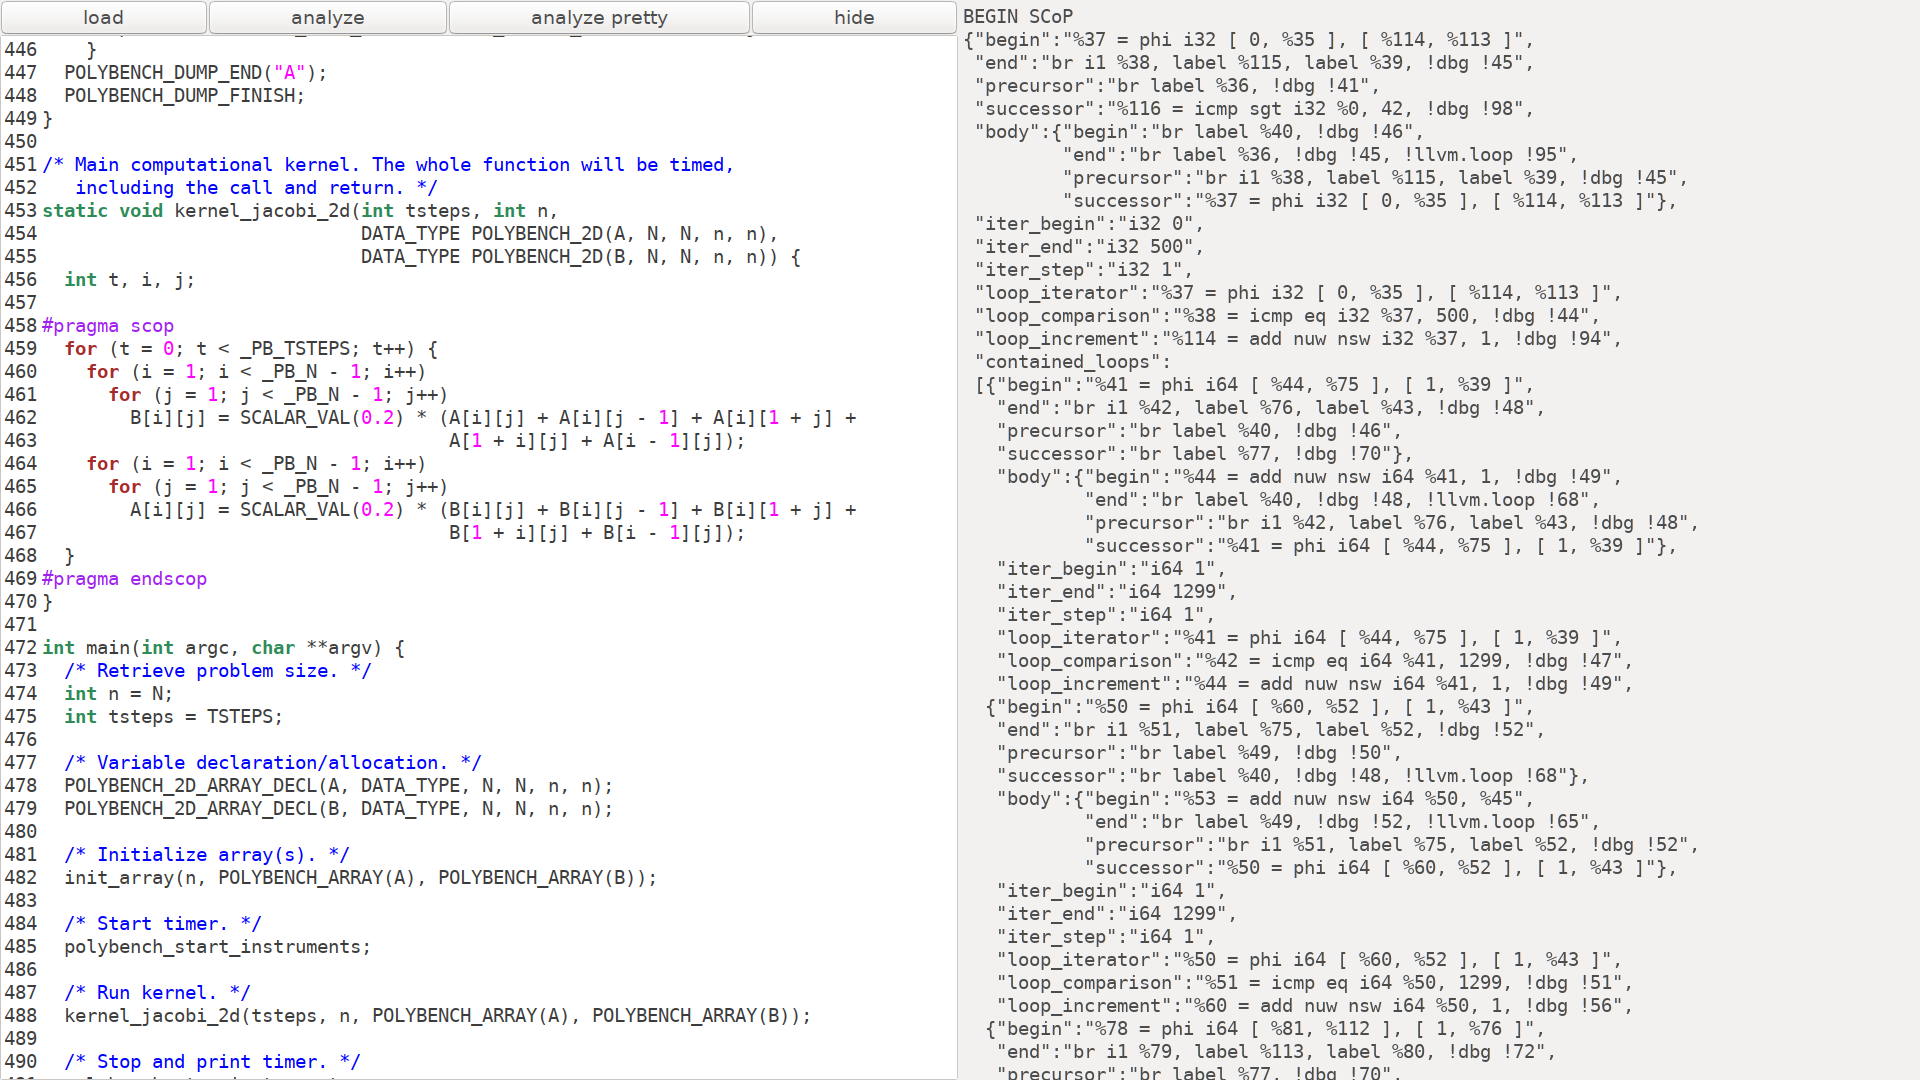
\includegraphics[width=\textwidth]{figures/visual_gui2.png}
\caption{Interactive CAnDL test tool}
\medskip
\small
Left hand panel shows a SCoP in Polybench jacobi-2d, the right hand panel show the corresponding constraint solution
\label{fig:gui}
\end{figure*}

\subsection{Developer Tools}

    CAnDL makes writing compiler analysis passes easier, but reasoning about the
    semantics of compiler IR still remains difficult and the correctness of
    CAnDL programs can only be guaranteed with thorough testing.
    It is important to keep in mind that CAnDL is targeted at expert compiler
    developers.

    In order to make debugging of CAnDL programs more feasible, several
    supporting tools can be used.
    Most importantly, this includes an interactive gui, where developers can
    test out corner cases of CAnDL programs to find false positives and false
    negatives.
    This gui is shown in \Cref{fig:gui}, the example is from one of the use
    cases presented in \Cref{sec:casestudies}.

    In the left column,  part of a C program from the PolyBench benchmark suite
    is visible, which implements a two-dimensional Jacobi stencil.
    The gui is configured to look for static control flow regions (SCoPs), as
    described later in one of the use cases.
    The user has clicked the ``analyze'' button, which triggered the analysis to
    run and prints the results in the right column.

    The solver found a SCoP in the IR code (corresponding to lines 459-468 of
    the C program).
    The text on the right shows the hierarchical structure of the solution, with
    IR values assigned to every variable.
    The corresponding C entities can be recovered using the debug
    information that is contained in the generated LLVM IR code.
    By modifying the C code, the developer can now test the detection and
    e.g.\ verify that no SCoP is detected if irregular control flow is
    introduced.

\section{Case Studies}
\label{sec:casestudies}

    The usefulness of CAnDL is evaluated on three real life use cases.
    First, it is used for simple peephole optimizations.
    Secondly, CAnDL is applied to graphics shader code optimisation.
    Finally, the detection of static control flow parts (SCoPs) for polyhedral
    code analysis is demonstrated.
    Where possible, the evaluation compares the number of lines of CAnDL code,
    the achieved program coverage and performance against prior approaches.

\subsection{Simple Optimizations}

    Arithmetic simplifications in LLVM are implemented in the
    \texttt{instcombine} pass.
    One example of this is the standard factorization optimization that uses the
    law of distributivity to simplify integer calculations as shown in
    \Cref{fig:factorization1}.
    It is implemented in 203 lines of code and furthermore uses supporting
    functionality provided by \texttt{instcombine}.
    \begin{align}
        a*b+a*c\rightarrow a*(b+c)
        \label{fig:factorization1}
    \end{align}
    This analysis problem can be formulated in CAnDL as shown in
    \Cref{fig:facopport}.
    Crucually, in lines 5,7,9,11, the specification makes use of
    \texttt{SumChain} and \texttt{MulChain}, which allows the CAnDL program
    to capture a large, generalised class of opportunities for factorization.
    The \texttt{instcombine} pass only has limited support for this, and
    requires to first apply associative and commutative laws to reorder the
    values.
    This is for example needed in the case of \Cref{fig:factorization2} and
    only partially supported by LLVM with the additional \texttt{reassociate}
    pass.
    \begin{align}
        a*b+c+d*a*e->a*(b+d*e)+c
        \label{fig:factorization2}
    \end{align}

\begin{figure}[t]
\begin{lstlisting}[language=CAnDL]
Constraint ComplexFactorization
( opcode{value} = add
([$\tt \land$]) {value}.args[0] = {sum1.value}
([$\tt \land$]) {value}.args[1] = {sum2.value}
([$\tt \land$]) include SumChain at {sum1}
([$\tt \land$]) {mul1.value} = {sum1.last_factor}
([$\tt \land$]) include MulChain at {mul1}
([$\tt \land$]) {mul1.last_factor} = {mul2.last_factor}
([$\tt \land$]) include SumChain at {sum2}
([$\tt \land$]) {mul2.value} = {sum2.last_factor}
([$\tt \land$]) include MulChain at {mul2})
End
\end{lstlisting}
\vspace{-0.3cm}
\caption{ComplexFactorization in CAnDL}
\label{fig:facopport}
\end{figure}

\subsubsection{Setup}

    The program in \Cref{fig:facopport} was evaluated against the default
    factorisation optimisation in LLVM's \texttt{instcombine} on three benchmark
    suites: the sequential C versions of NPB, the C versions of Parboil and the
    OpenMP C/C++ versions of Rodinia.
    The existing LLVM \texttt{instcombine} pass was extended so that it
    automatically reports every time that it successfully applies the
    \texttt{tryFactorization} function.  

    % NPB:     29047 loc
    % Parboil:  7358 loc
    % Rodinia: 58510 loc
    The individual benchmark programs in the three benchmark
    suites consist of 94915 lines of code in total.
    For each benchmark suite, the total number of reported factorisations as
    well as LLVM's total compilation time were measured.

    Then the standard LLVM optimisation was disabled and instead the CAnDL
    generated detection functionality was used.
    The same application programs were compiled, reporting the number of
    factorisations found, and again measuring the total compilation time.
    Note that this compilation time includes all the other passes within LLVM as
    well as the CAnDL generated path.

\subsubsection{Results}

\begin{figure}[b]
\centering
\begin{tabular}{|l||l|l|}
\hline
         & LLVM  &CAnDL \\
\hline
\hline
Lines of Code & 203 & 12 \\ \hline
Detected in NPB & 1 & 1 + 2 \\
Detected in Parboil & 0 & 0 + 1\\
Detected in  & 24 & 24 + 4\\ \hline
Total Compilation time & 152.2s & 152.2s+7.8s \\ \hline
\hline
\end{tabular}
\vspace{-0.1cm}
\caption{Factorizations LLVM vs CAnDL}
\label{fig:factorization_results}
\end{figure}

    The results are shown in \Cref{fig:factorization_results}.
    In general, the performance impact of peephole optimizations is small
    and in two of the benchmark sets we find only very small numbers.
    LLVM was unable to perform any factorisation in the entire Parboil suite.
    However, the Rodinia suite contains more opportunities, mostly in the
    Particlefilter and Mummergpu programs.

    In all three benchmarks suites, our scheme finds the same factorization
    opportunities as the \texttt{instcombine} pass plus an additional 7 cases.
    With only 12 lines of CAnDL code, we were able to capture more factorization
    opportunities than LLVM did using two hundred lines of code.

    Using CAnDL on large complex benchmark suites only increased total
    compilation time by 5\%, demonstrating its use as a prototyping tool.

\subsection{Graphics Shader Optimizations}

\begin{figure}[t]
\begin{lstlisting}[language=CAnDL]
Constraint FloatingPointAssociativeReorder
( include VectorMulChain and
([$\tt \land$]) collect j N
([$\tt \land$]) ( {hoisted[k]} = {factors[i]} forsome i=0..N
  ([$\tt \land$]) include ScalarHoist({hoisted[j]}->{out},
                       {scalar[j]}->{in})@{hoist[j]})
([$\tt \land$]) collect j N
  ( {nonhoisted[j]}  = {factors[i]} forsome i=0..N
  ([$\tt \land$]) {nonhoisted[j]} != {hoisted[i]} forall  i=0..N))
End
\end{lstlisting}
\vspace{-0.3cm}
\caption{CAnDL code for vectorized multiplication chains}
\label{fig:Lewis}
\end{figure}

    Graphics computations often involve arithmetic on vectors of single
    precision floating point values that represent either vertex positions in
    space or color values.
    Common graphics shader compilers utilize the LLVM framework internally.
    The LunarGLASS project was used in this work as an open source
    implementation of LLVM for graphics shaders.

    There are opportunities for associative reordering that LLVM misses.
    In general purpose code, such reordering can be problematic due to floating
    point computation artifacts.
    However, this is not a problem in the domain of graphics processing.
    Under specific circumstances, associative reordering within computations
    that mixes vector and scalar arithmetic can result in real performance
    improvements.

%    For real shader code, LLVM misses an opportunity for the associative
%    reordering of floating point computations.
%    Although such reordering is problematic in general, it is applicable in the
%    domain of graphics processing.

    There are often products of multiple floating point vectors, where several
    of the factors are actually scalars that were hoisted to vectors.
    By reordering the factors and delaying the hoisting to vectors, some of the
    vector products can be simplified to scalar products, as shown in the
    following equation.
    \begin{align*}
        \vec x={}&\vec a*_v\vec b*_v\text{vec3}(c)*_v\vec d*_v\text{vec3}(e)\\
        ={}&\text{vec3}(c*e)*\vec a*_v\vec b*_v\vec d
    \end{align*}

    The required analysis functionality for this optimization was implemented
    with CAnDL, as shown in \Cref{fig:Lewis}.
    The \mbox{included} \texttt{VectorMulChain} subprogram discovers chains of
    floating point vector multiplications in the IR code and uses the variables
    \texttt{factors} and \texttt{partials} such that the following equations
    hold
    \begin{align*}
        \text{\tt partials}[0] &= \text{\tt factors}[0]\\
        \text{\tt partials}[i+1] &= \text{\tt partials}[i]\times\text{\tt factors}[i+1].
    \end{align*}
    The \texttt{VectorMulChain} program furthermore guarantees that this is a
    chain of maximal length by checking that neither of the first two factors
    are multiplications and the last factor is not used in any multiplication.
    \texttt{ScalarHoist} detects the hoisting of scalars to vectors and this is
    used to collect all hoisted factors into the array \texttt{hoisted}.
    In a last step, all other factors are collected into the array
    \texttt{nonhoisted}.

    The corresponding transformation pass simply generates all the appropriate
    scalar and vector multiplications and replaces the old result with this
    newly generated one.
    We evaluated the performance impact on the CFXBench 4.0 on the  Qualcomm
    Adreno 530 GPU.

\subsubsection{Results}

\begin{figure}[t]
\centering
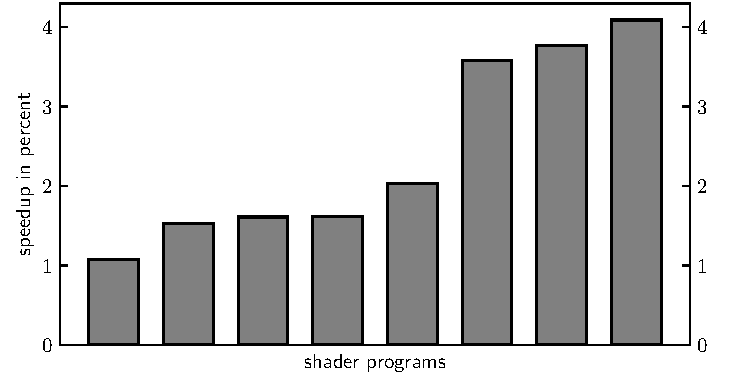
\includegraphics[width=\linewidth]{figures/qualcomm_plot.pdf}
\caption{Speedup on Qualcomm Adreno 530}
\label{fig:qualcommspeedup}
\end{figure}

\begin{figure}[b]
\centering
\begin{tabular}{|l||l|l|}
\hline
         & LLVM  &CAnDL \\
\hline
\hline
Lines of Code & Not implemented& 10 \\ \hline
Detected in GFX 4.0 & - & 19 \\ \hline
\hline
\end{tabular}
\caption{Shader optimization LLVM vs CAnDL}
\label{fig:candlshader}
\end{figure}

    The optimization was relevant to 8 of the fragment shaders in GFXBench 4.0.
    The number of lines of code needed and the resulting performance impact are
    shown in \Cref{fig:candlshader} and \Cref{fig:qualcommspeedup}.
    A total of 19 opportunities for the optimization to be applied were
    detected.
    Although the performance impact was moderate with $1-4\%$ speedup on eight
    of the fragment shaders, it shows how new analysis can be rapidly prototyped
    and evaluated with only a few lines of code.

\subsection{Polyhedral SCoPs}

    The polyhedral model allows compilers to utilize powerful mathematical
    reasoning to detect parallelism opportunities in sequential code and to
    implement code transformations for well structured nested
    loops.
    It is currently applicable to Static Control Flow Parts (SCoPs) with affine
    data dependencies.
    Detecting SCoPs is fundamental and a necessary first step for any later
    polyhedral optimization.

    Implementations of the polyhedral model may differ in their precise
    definition of SCoPs.
    In this work, the definition of Semantic SCoPs in \citet{Lengauer2012Polly}
    was used for reference.
    SCoP detection functionality was implemented in CAnDL and compared against
    the Polly implementation in LLVM.
    The complete CAnDL code for this section is in Appendix~\ref{appendix:CAnDL}.
    The constraints for SCoPs can be broken into several components:

    \paragraph*{Structured Control Flow}
    SCoPs require well structured control flow.
    Technically speaking, this means that every conditional jump within the
    corresponding piece of IR is accounted for by for loops and conditionals.
    This is enforced with the \texttt{collect} statement that was introduced in
    \Cref{fig:collectexample}.
    It is used in CAnDL programs \texttt{ForLoop} and
    \texttt{Conditional} that describe the control flow of for loops and
    conditionals and extract the involved conditional jump instructions.
    Another \texttt{collect} is then used to verify that these are indeed all
    conditional jumps within the potential SCoP.

    Once the control flow has been established, the iterators that are
    involved in the loops are used to define affine integer computations in the
    loop.
    This is done in a brute force fashion with a recursive constraint program.
    Using this analysis we then check that the iteration domain of all the for
    loops is well behaved, i.e.\ the boundaries are affine in the loop
    iterators.

    \paragraph*{Affine Memory Access}
    All memory access in the SCoP has to be affine.
    For this to be true, it needs to be verified that for each load and store
    instruction, the base pointer is loop invariant and the index is calculated
    affinely.
    The loop invariant base pointer is easily guaranteed using the
    \texttt{LocalConst} program from \Cref{fig:localconstant}.

    Checking the index calculations is more involved and is again based on the
    \texttt{collect} method that was demonstrated in \Cref{fig:collectexample}.
    The \texttt{collect} construct is used to to find all of the affine memory
    accesses in all the loop nests.
    We then use collect all \texttt{load} and \texttt{store} instructions and
    verify that both collections are identical.

\subsubsection{Setup}

    The detection of SCoPs was evaluated on the PolyBench suite.
    For both the CAnDL based approach as well as for Polly, it was counted
    counted how many of the computational kernels contained in the benchmark
    suite are captured by the analysis.

\subsubsection{Results}

    As is visible in \Cref{fig:candlvspolly}, the CAnDL program captured all
    the SCoPs that Polly was able to detect.
    There is some postprocessing of the generated constraint solutions required
    to achieve this.
    Firstly, the CAnDL results are not in the jscop format that Polly uses but
    contain the raw constraint solution as shown on the right side of
    \Cref{fig:gui}.
    Also, the CAnDL implementation does not merge consecutive outer level loops
    into SCoPs of maximum size.
    To compare, the detected loops from the CAnDL solver were extracted and then
    grouped them into maximum size SCoPs.
    It was then manually verified that they fully cover the SCoPs detected by
    Polly.

    To measure lines of code, we compared our version with the amount of code in
    Polly's \texttt{ScopDetection.cpp} pass.
    We are able to detect the same number of SCoPs with much fewer lines of
    code.
    Note that the LoC count that we give for our SCoP program does not include
    all CAnDL code involved in the detection of polyhedral regions.
    We consider the code that is not specific to this idiom (such as loop
    structures) to be part of the CAnDL standard library.
    In the same way we did not account for e.g\ the ScalarEvolution pass when
    counting the lines for Polly.

    By having a high level representation of SCoPs, we allow polyhedral compiler
    researchers to explore the impact of relaxing or tightening the exact
    definition of SCoPs in a straightforward manner, enabling rapid prototyping.

\begin{figure}[ht]
    \centering
\begin{tabular}{|l||l|l|}
\hline
         & Polly & CAnDL \\
\hline
\hline
Lines of Code & 1903 & 45 \\ \hline
Detected in datamining & 2 & 2\\
Detected in Linear-algebra & 19 & 19\\
Detected in medley & 3 & 3\\
Detected in stencils & 6 & 6\\ \hline
%Compilation time & 24.4s+37.5s & 24.4s+12.7s \\ \hline
\end{tabular}
    \label{fig:candlvspolly}
\end{figure}

\section{Summary}

    Optimising compilers require sophisticated program analysis in order to
    generate performant code.
    The current way of implementing this functionality manually in programming
    languages such as C++ is not satisfactory.

    The domain specific Compiler Analysis Description Language (CAnDL) provides
    a more efficient approach.
    CAnDL programs can be used to automatically generate compiler analysis
    passes.
    They are easier to write and reduce the code size and complexity when
    comparing against manual C++ implementations.

    Although CAnDL is based on a constraint programming paradigm and uses a
    backtracking solver to analyze LLVM IR code, the use of CAnDL results in
    only moderate compile time increases.
    Many compiler analysis tasks are suitable for CAnDL, from
    peephole optimisations to sophisticated program analysis with the polyhedral
    model.
